\section{Results}
\label{sec:results}

The comparison is scoped to the two BEAM tiers for which Mem0 publishes per-question answers, scored by one judge for both systems, and to retrieval alone on LongMemEval-S.

\subsection{BEAM}
\label{sec:beam}

Under one judge, base retrieval passes 64.7\% of the 700 questions and Mem0 63.9\%, a gap of $+0.9$ with interval $[-3.0, +4.4]$: a tie (Figure~\ref{fig:lead}). The full method passes 67.3\%, 3.4 points above Mem0, with interval $[-0.4, +7.3]$. That interval also includes zero, so we report a tie here too (Figure~\ref{fig:abilities}; Table~\ref{tab:beam} has the numbers). Resampling the same conversations on both sides gives a paired interval of $[+0.3, +6.6]$; we registered the independent form and keep the tie.

\begin{figure}[t]
\centering
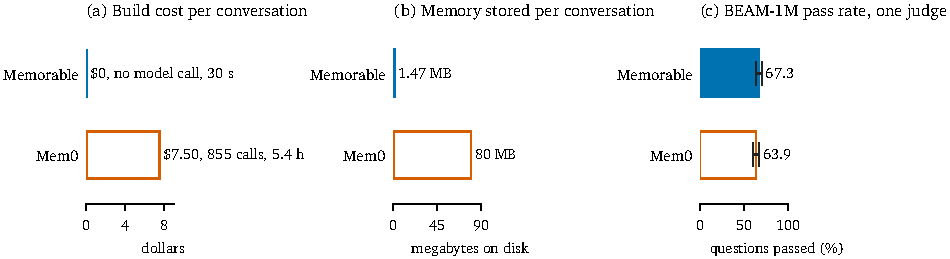
\includegraphics[width=\textwidth]{fig_lead3.pdf}
\caption{Build cost, bytes stored and pass rate for one 1M-token BEAM conversation. Left: model cost, calls and time to build the memory, measured on Mem0's open-source release over 80\% of the conversation and extrapolated to the whole. Middle: bytes stored on disk. Right: pass rate on BEAM-1M under one judge, 700 questions, with 95\% Wilson intervals. Per-question cost is in Figure~\ref{fig:breakeven}.}
\label{fig:lead}
\end{figure}

\begin{figure}[t]
\centering
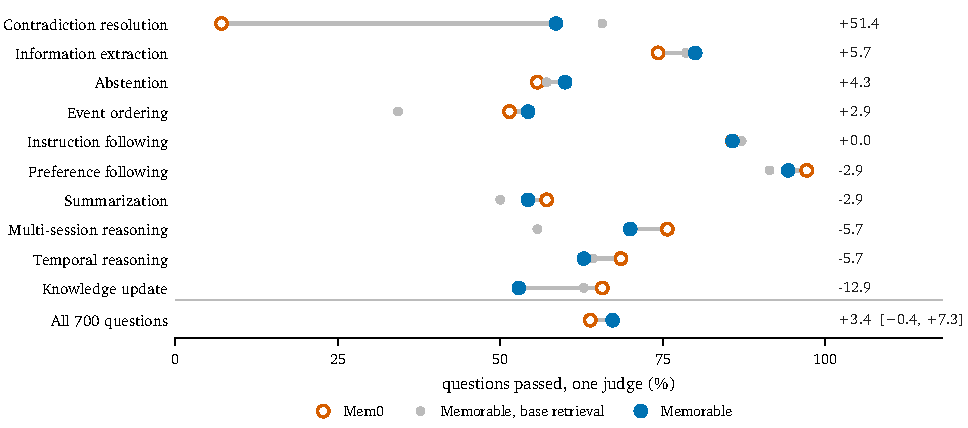
\includegraphics[width=\textwidth]{fig_abilities.pdf}
\caption{BEAM-1M by ability, one judge, 70 questions per ability. Hollow dots are Mem0, filled blue dots are Memorable and small grey dots are base retrieval. The grey line joins Mem0 to Memorable; the number at the right is Memorable minus Mem0 in points. The last row is all 700 questions with the bootstrap interval on the gap.}
\label{fig:abilities}
\end{figure}

\paragraph{Contradiction questions.} The largest gap between the two systems is here. These questions ask about a fact the user changed, and the rubric asks the answer to name both statements. In the first conversation the user writes ``I've completed the translation microservice and it's working great'' and, 158 turns later, that they have never completed it. Our reader sees both turns and says so: under the one judge the full method passes 58.6\% of these questions and base retrieval 65.7\%, against 7.1\% for Mem0. The gap holds under both judges that scored both systems, and its size varies with the judge. Mem0's own judge scores the same answers 48.6\% and BEAM's judge 15.7\%, and under BEAM's judge base retrieval scores 64.3\% and the full method 42.9\% (Appendix~\ref{app:ownjudge}). In Mem0's open-source release an UPDATE replaces the earlier fact, so the memory holds one version. Its hosted pipeline is closed, so we cannot confirm that the same step produced the 7.1\%.

\paragraph{What search adds.} Base retrieval trails Mem0 on the abilities whose evidence is spread over several sessions: multi-session reasoning by 20.0 points, event ordering by 17.1 and summarization by 7.1. One query finds one session, whereas a memory that a model wrote holds facts from every session in one store. The planner, the 60-turn read and the session cap are aimed at this gap. On the development sets (400 questions pooled over the 100K and 500K tiers, gpt-5-mini reader, BEAM's judge) they raise the pass rate from 74.2\% to 79.8\%, with multi-session reasoning moving from 67.5 to 82.5, event ordering from 52.5 to 70.0 and summarization from 65.0 to 80.0 (Figure~\ref{fig:ladder}). On the 1M tier under one judge the same components move multi-session reasoning from 55.7 to 70.0, event ordering from 34.3 to 54.3 and summarization from 50.0 to 54.3. They cost ground on two abilities: knowledge update falls from 62.9 to 52.9 and contradiction resolution from 65.7 to 58.6, and under BEAM's judge the contradiction drop is larger, 64.3 to 42.9. Of the 18 contradiction questions lost under that judge, half dropped a gold turn from the read set; in the other half the reader listed both statements as a dated timeline and left their conflict unnamed. The rubric requires the conflict to be named (Appendix~\ref{app:ownjudge}).

\paragraph{Where Mem0 stays ahead.} Mem0 leads on knowledge update by 12.8 points, and by 2.9 to 5.7 points, two to four questions of 70, on temporal reasoning, multi-session reasoning, preference following and summarization (Figure~\ref{fig:abilities}). Knowledge-update questions ask for the current value of a fact that changed. A memory that overwrites holds only that value, whereas our reader sees both turns and has to pick the later one; we did not test whether this explains the gap.

\begin{figure}[H]
\centering
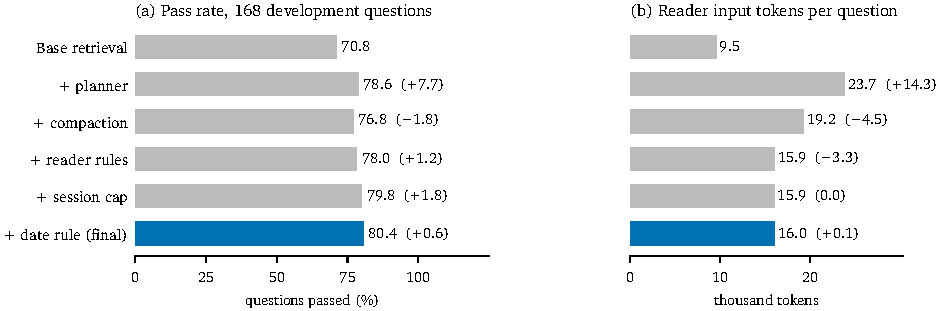
\includegraphics[width=\textwidth]{fig_ladder.pdf}
\caption{Adding the search components one at a time on the 500K development tier (development questions, separate from the 1M result): 168 questions every run answered, gpt-5-mini reader, BEAM's judge. Left: pass rate. Right: input tokens handed to the reader per question. The planner adds 7.7 points and 14.3K tokens; compaction and the reader rules return 7.8K of those tokens.}
\label{fig:ladder}
\end{figure}

\paragraph{The 10M tier.} Mem0 publishes answers for the ten conversations of BEAM's 10M-token tier, 200 questions, and we ran the full method on them once after registering predictions (Appendix~\ref{app:predictions}). Under the one judge Memorable passes 56.0\% and Mem0 46.5\%, a gap of 9.5 points with a registered interval of $[+0.5, +18.0]$ and a paired interval of $[+7.0, +12.0]$ (Figure~\ref{fig:abilities10m}). Memorable is ahead in each of the ten conversations, by one to three questions of 20; with all ten differences positive, a two-sided sign-flip test gives $p = 2/1024 = 0.002$. Contradiction resolution is 60.0\% against 10.0\% and temporal reasoning 50.0\% against 20.0\%, while Mem0 stays ahead on preference following, 90.0\% against 75.0\%, and on multi-session reasoning, 30.0\% against 25.0\%. Each ability has 20 questions here, so one question moves it by 5 points, and temporal reasoning changes sign between tiers (Mem0 ahead by 5.7 points on 1M, Memorable ahead by 30.0 here); we do not interpret that. The reader took 16,172 input tokens per question, and the run cost \$10.21, of which \$9.49 was the reader and the rest the planner and BEAM's judge in the run loop. The memory of a 10M-token conversation takes 16.7~MB, above the 10~MB we predicted.

\begin{figure}[H]
\centering
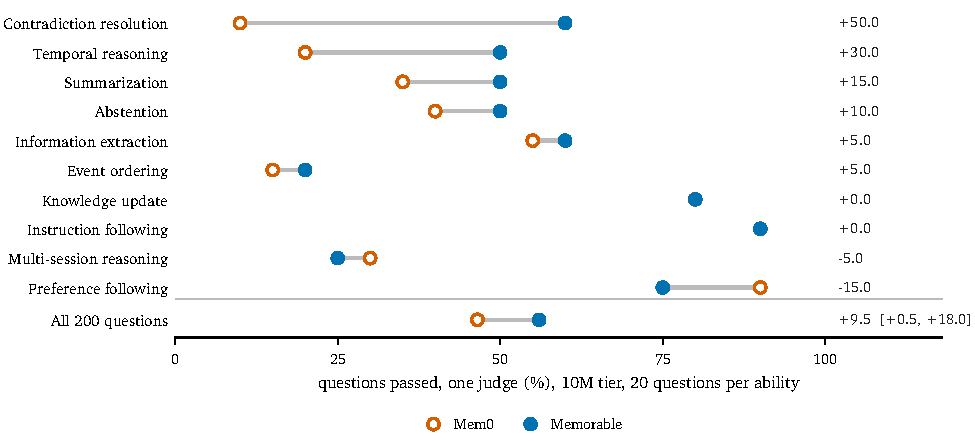
\includegraphics[width=\textwidth]{fig_abilities_10m.pdf}
\caption{BEAM-10M, 200 questions over ten conversations, one judge. Hollow orange: Mem0 (Platform v3, GPT-5). Filled blue: Memorable, full method with the 1M settings, run once. Right: the gap in points; the interval beside the All 200 questions row is the registered 95\% interval.}
\label{fig:abilities10m}
\end{figure}

\subsection{Cost and storage}
\label{sec:cost}

\paragraph{Build.} Building the memory of the first 1M conversation with Mem0's open-source release and gpt-5-mini as extractor took 683 extraction calls for 80\% of the turns before a \$6 cap stopped it: 6.85M input and 2.14M output tokens, 3,788 memory entries, 260 minutes at one worker and 64~MB on disk. Scaled to the whole conversation, that is about 855 calls, \$7.50, 5.4 hours and 80~MB (Table~\ref{tab:build}). Memorable builds the same conversation in about 30 seconds of CPU and stores 1.47~MB, 0.81~MB of compressed text and 0.66~MB of 8-bit vectors (Figure~\ref{fig:waterfall}). Mem0's facts take less text than our turns: about 4,700 entries for the whole conversation hold 1.15~MB against our 3.67~MB of compacted turns before compression, or 0.34~MB against 0.81~MB after zlib. Each entry also carries a float vector, 2.8 per turn and 7.3~MB in all, and the rest of the 80~MB is its vector database and index.

\begin{figure}[H]
\centering
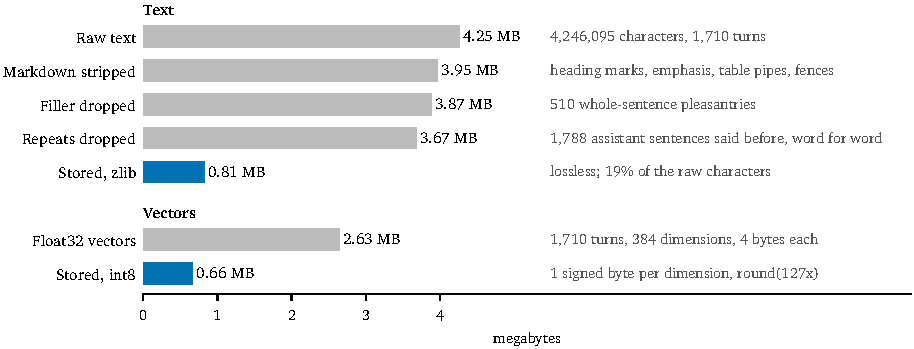
\includegraphics[width=\textwidth]{fig_waterfall.pdf}
\caption{Bytes kept at each step for the first 1M conversation. Text: raw, after each compaction rule, and after zlib. Vectors: float32 and 8-bit.}
\label{fig:waterfall}
\end{figure}

\paragraph{Per question.} Memorable's reader, GPT-5, takes 17,200 input tokens and produces 2,450 output tokens per question, \$0.046 at GPT-5 prices measured over the 700 questions, plus about \$0.001 for the planner call. Mem0's reader takes 200 facts of about 242 characters, about 12,100 input tokens, plus about 450 for the question and instructions. Mem0 publishes the facts and leaves out token counts, so we assume 1,500 output tokens; GPT-5 prices then give \$0.0307, which we write as \$0.031. With Equation~\ref{eq:cost} the two systems cost the same after about 460 questions on one conversation (Figure~\ref{fig:breakeven}).

\begin{figure}[H]
\centering
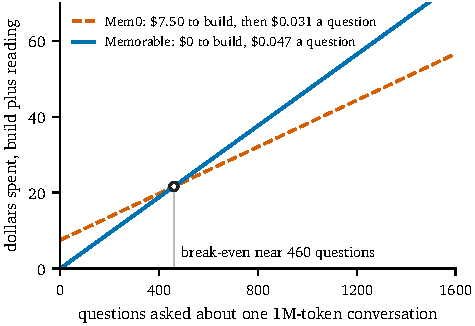
\includegraphics[width=0.55\textwidth]{fig_breakeven.pdf}
\caption{Dollars spent on one 1M-token conversation as questions accumulate. Mem0 starts at its measured build cost; Memorable starts at zero. Mem0's per-question cost is estimated from the size of its retrieved facts; ours is measured.}
\label{fig:breakeven}
\end{figure}

\subsection{LongMemEval-S}
\label{sec:lme}

\paragraph{Retrieval.} Keyword and embedding rankings fused by reciprocal rank and rescored by the cross-encoder place every gold session in the top 10 for 95.5\% of the 375 LongMemEval-S test questions with gold labels. EdgeMem reports 93.8\% and MemGAS 94.5\% \citep{cui2026edgemem,xu2025memgas}, and we read the published metrics as the same measure. The 95 development questions, on which we made the retrieval choices, score 92.6\%; all 470 together score 94.9\%. On LongMemEval-S most gold turns are the user's, so a rule that hands the reader every user turn in the top 60, and an assistant reply only when it ranks in the top 10, brings the input to 6,777 tokens and keeps every gold turn for 97.9\% of development questions. We have not run a reader on that setting.
